\section{МДМ фальш-сигнал} \label{sec:simulation-fake_signal}
Данная серия симуляций была проведена с целью подтвердить два тезиса
касательно систематической ошибки измерения частоты прецессии спина в
вертикальной плоскости, вызванной неточностью установки E+B элементов:
\begin{enumerate*}[1)]
	\item индуцированный МДМ-эффект зависит только от среднего значения
	угла наклона элементов, но не от  конкретной последовательности
	углов (т.е. отсутствует эффект \emph{геометрической фазы}); и
	\item эта зависимость носит линейный характер.
\end{enumerate*}

Наклон элемента вокруг оптической оси моделировался путём добавления
после элемента спин-кика вокруг радиальной оси соответствующей
величины (см. раздел~\ref{sec:error_field_implementation}). Это
гарантирует сохранение замкнутой орбиты при введении наклонов, что
физически обусловлено появлением компенсирующего электрического поля 
спин-ротатора при его наклоне.

Симуляция была проведена следующим образом: мы распределили наклоны
$\Theta_{tilt}$ E+B элементам FS структуры случайным образом. После
построения матриц перехода 3-го порядка, были вычислены разложения
Тейлора функций спин-тюна и оси прецессии спина (SPA). Члены нулевого
порядка этих разложений представляют собой спин-тюн и SPA референсной частицы.

Симуляция была проведена 11 раз; каждый раз углы наклона
спин-ротаторов выбирались из нормального распределения
$N(\mu_0\cdot(i-5), \sigma_0)$, где $\mu_0 = 10\cdot \sigma_0 =
10^{-4}$ рад, $i\in\lbrace0,\dots, 10\rbrace$. Результаты представлены
на Рисунке~\ref{fig:Linearity_test_shifting_gauss}.

\begin{figure}[!h]
	\centering\hfill
	\subbottom[Компоненты оси прецессии.]{%
		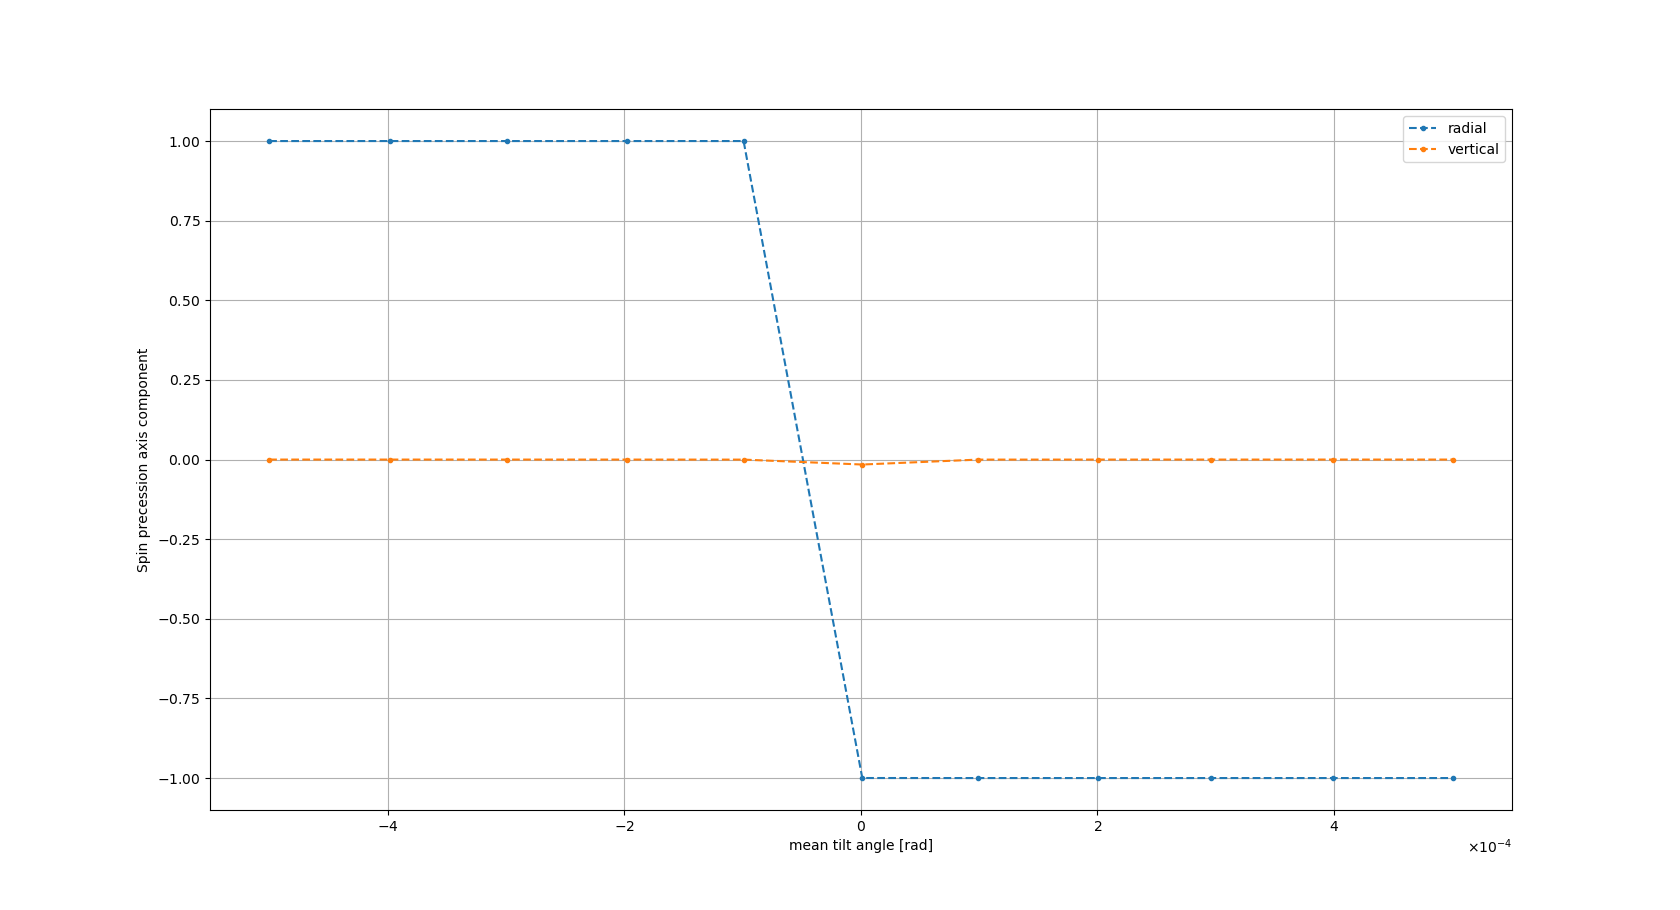
\includegraphics[width=\textwidth]{images/fake_signal_sim/linearity_test_shifting_gauss_nbar}}
	\hfill
	\subbottom[Компоненты частоты прецессии.]{%
		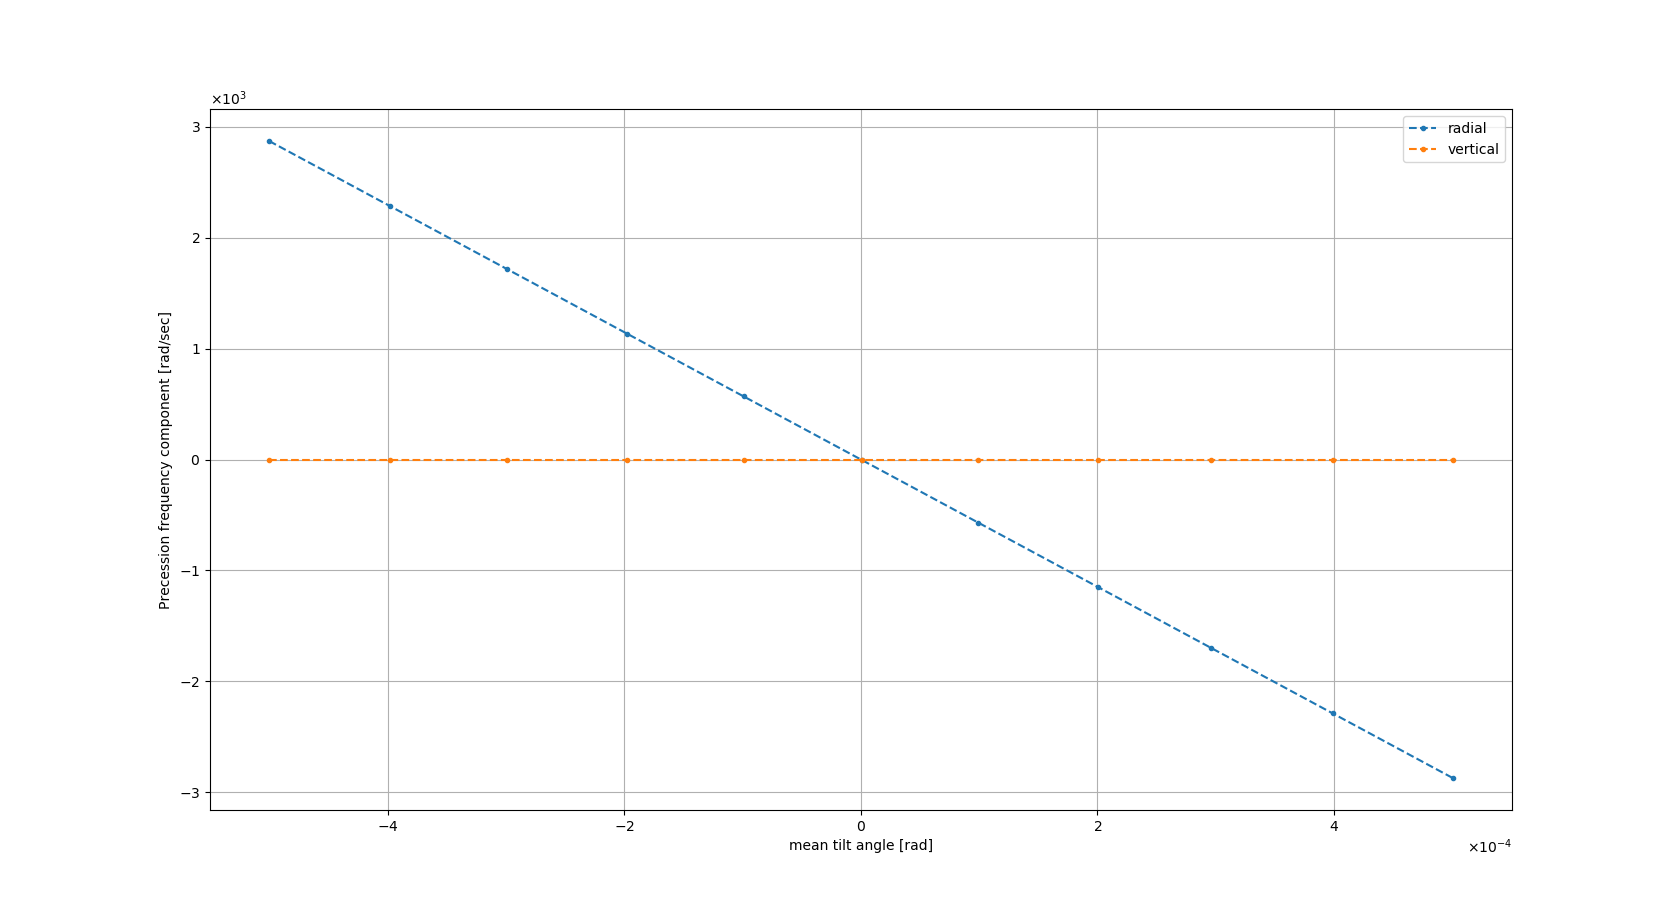
\includegraphics[width=\textwidth]{images/fake_signal_sim/linearity_test_shifting_gauss_freq}}
	\hfill
	\legend{Цветом различаются радиальная (синий) и вертикальная (оранжевый) компоненты векторов $\bar n$, $\vec\W$.}
	\caption{Зависимость направления и частоты прецессии спина референсной частицы в неидеальной FS-структуре со случайно распределёнными ошибками установки спин-ротаторов от их среднего угла наклона. (Случайно распределённая ошибка установки.)\label{fig:Linearity_test_shifting_gauss}}
\end{figure}

На Рисунке~\ref{fig:Linearity_test_compensated} изображены результаты теста, в котором E+B элементы попарно повёрнуты на противоположные углы (три случайные пары), а один элемент повёрнут на угол
$\mu_i = (i-5)\cdot 10^{-6}$ рад, $i\in\lbrace0,\dots,10\rbrace$. Обе симуляции были выполнены на энергии
270.0092 МэВ.\footnote{На этой энергии ось прецесии спина и спин-тюн
	не определены в системе координат связанной с пучком, использованной
	COSY INFINITY, для идеальной структуры. Это соответствует ситуации
	когда спин не прецессирует ни в какой плоскости (горизонтальной или
	вертикальной), что есть условие замороженного спина в идеальной структуре.}

\begin{figure}[!h]
	\centering\hfill
	\subbottom[Компоненты оси прецессии]{%
		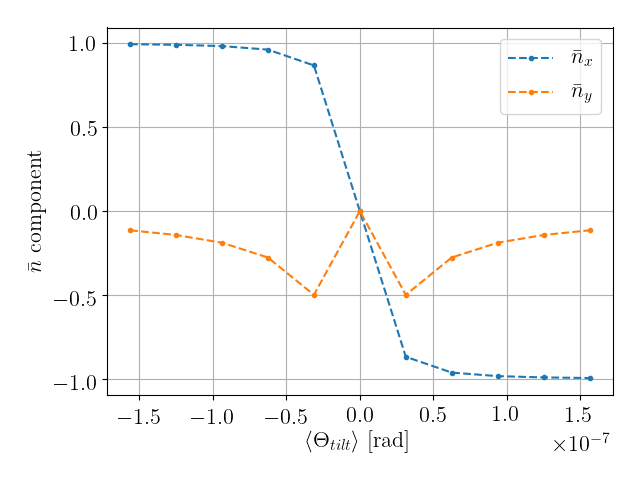
\includegraphics[width=\textwidth]{images/fake_signal_sim/linearity_test_compensated+microrad_nbar}}
	\hfill
	\subbottom[Компоненты частоты прецессии]{%
		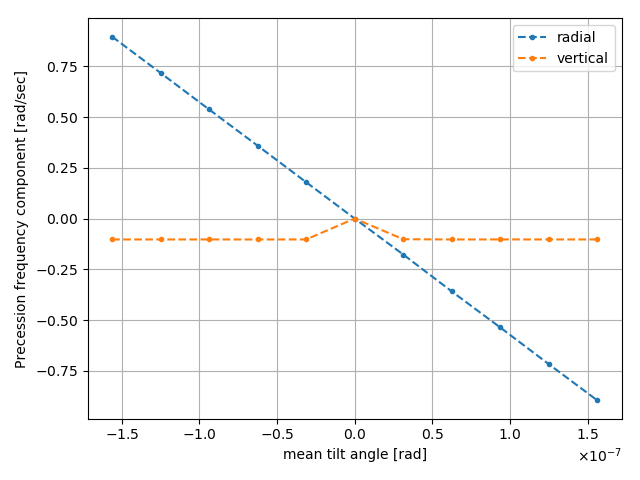
\includegraphics[width=\textwidth]{images/fake_signal_sim/linearity_test_compensated+microrad_freq}}
	\hfill
	\legend{Цветом различаются радиальная (синий) и вертикальная (оранжевый) компоненты векторов $\bar n$, $\vec\W$.}
	\caption{Зависимость направления и частоты прецессии спина референсной частицы в неидеальной FS-структуре со случайно распределёнными ошибками установки спин-ротаторов от их среднего угла наклона. (Скомпенсированная ошибка установки.)\label{fig:Linearity_test_compensated}}
\end{figure}